\documentclass[tikz]{standalone}
\usepackage{pgfplots}
\pgfplotsset{compat=1.15}
\usepackage{mathrsfs}
\usetikzlibrary{arrows,calc}
\usepackage{tkz-euclide}
\pagestyle{empty}

\definecolor{AngleClr}{rgb}{0,0.39215686274509803,0}
\definecolor{ShapeClr}{rgb}{0.6,0.2,0}

\begin{document}

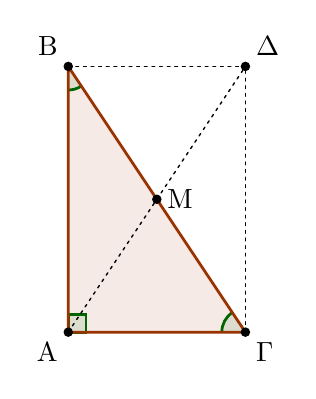
\begin{tikzpicture}[scale=.75]
\tkzSetUpLine[line width=1pt,color=black]
\tkzSetUpPoint[fill=black]

\tkzDefPoints{0/0/A,0/4.5/B,3/0/C,3/4.5/D}

\tkzFillPolygon[fill=ShapeClr,fill opacity=0.1](A,B,C)
\tkzMarkRightAngle[line width=1pt, size=.3,color=AngleClr,fill=AngleClr,fill opacity=0.1](B,A,C)
\tkzFillAngles[fill=AngleClr,size=.4,fill opacity=0.1](A,B,C B,C,A)
\tkzMarkAngles[line width=1pt,size=.4,color=AngleClr](A,B,C B,C,A)

\tkzDrawPolygon[color=ShapeClr](A,B,C)

\tkzLabelPoint[below left](A){$\rm A$}
\tkzLabelPoint[above left](B){$\rm B$}
\tkzLabelPoint[below right](C){$\rm \Gamma$}
\tkzLabelPoint[above right](D){$\rm \Delta$}

\tkzDefMidPoint(B,C) \tkzGetPoint{M}

\tkzDrawPoints[size=3](A,B,C,D,M)

\tkzLabelPoint[right](M){$\rm M$}


\tkzDrawSegments[line width=0.5pt,color=black,dashed,dash pattern=on 1pt off 1.75pt](A,D B,D C,D)

\end{tikzpicture}

\end{document}
